%!TEX root = main.tex

The evaluation and results of the metrics defined in section~\ref{cap:sec4} is presented in this section. We highlight the most useful metrics, however a previous and complete statistical analysis of the variables in the dataset have been performed. I.e., over 93\% of the BNI attempts are comming from China,

\subsection{BN propagation}
\begin{figure}[h]
    \label{fig:agg_grow}
    \caption{BN growth}
    \centering
    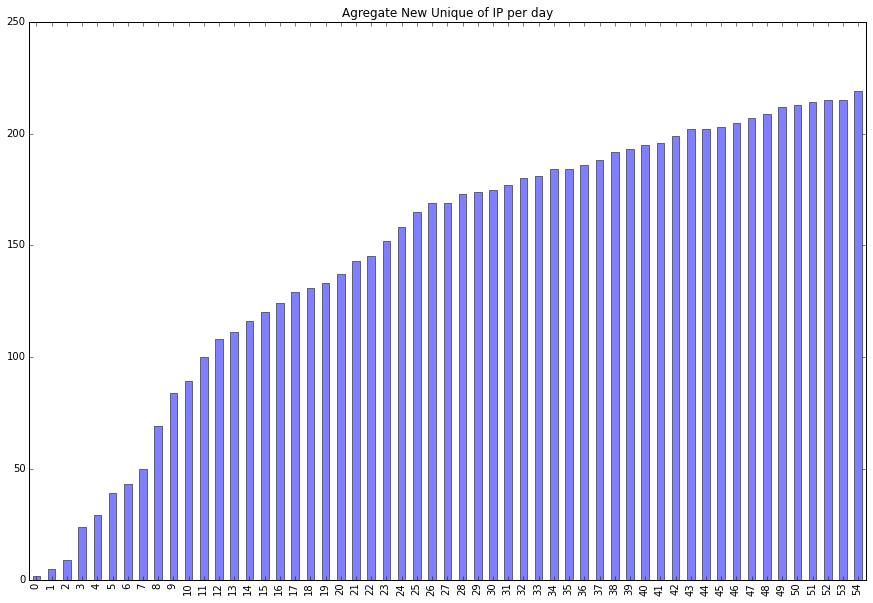
\includegraphics[width=\linewidth]{images/a_new_ip_da}
\end{figure}


\begin{figure*}[ht]
    \begin{subfigure}[ht]{0.5\linewidth}
        \caption{Unique IP per day}
        \centering
        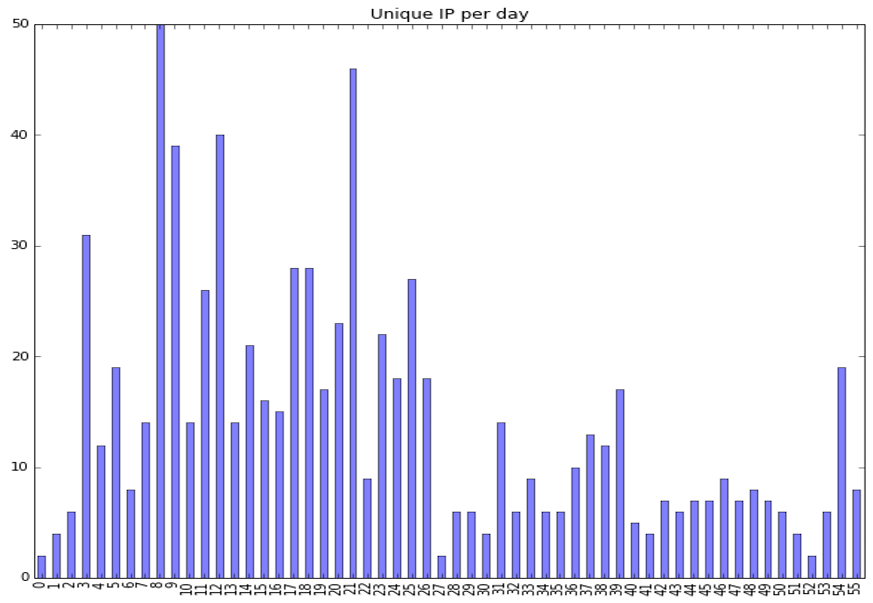
\includegraphics[width=\textwidth]{images/uni_ip_day}
    \end{subfigure}
\quad
    \begin{subfigure}[ht]{0.5\textwidth}
        \caption{BNI attempts}
        \centering
        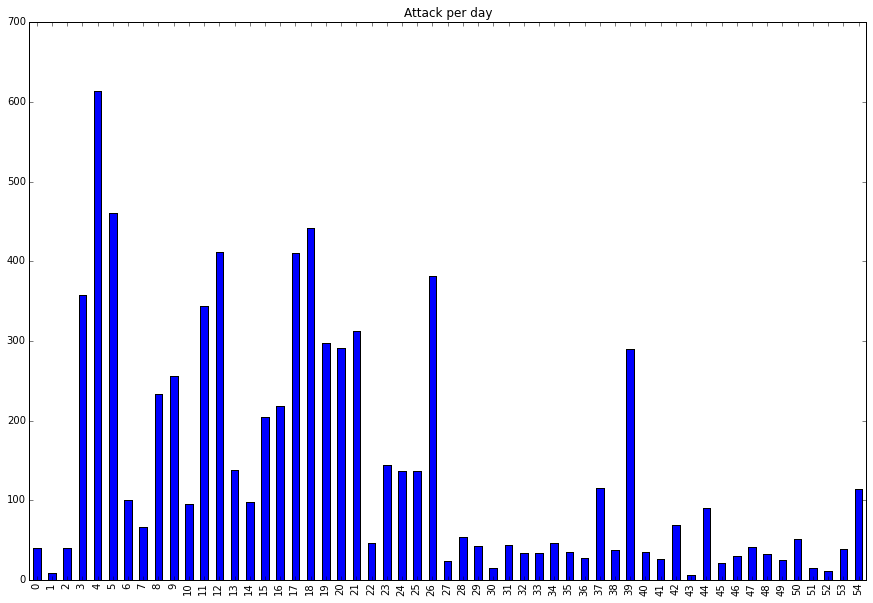
\includegraphics[width=\linewidth]{images/att_day}
    \end{subfigure}

\end{figure*}


\subsection{Network infection rate}
\begin{figure}[h]
    \caption{Subnet 218.10.0.0 attacks}
    \centering
        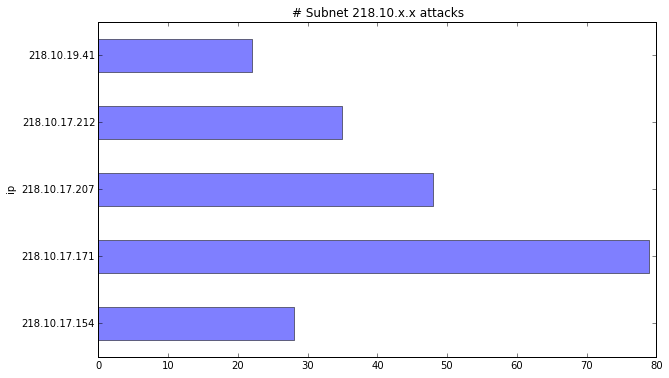
\includegraphics[width=0.9\linewidth]{images/subnet}
\end{figure}

\subsection{BN geographical and digital location.}
\begin{figure*}[h]
\caption{BNI geolocation~\cite{map}}
\centering
    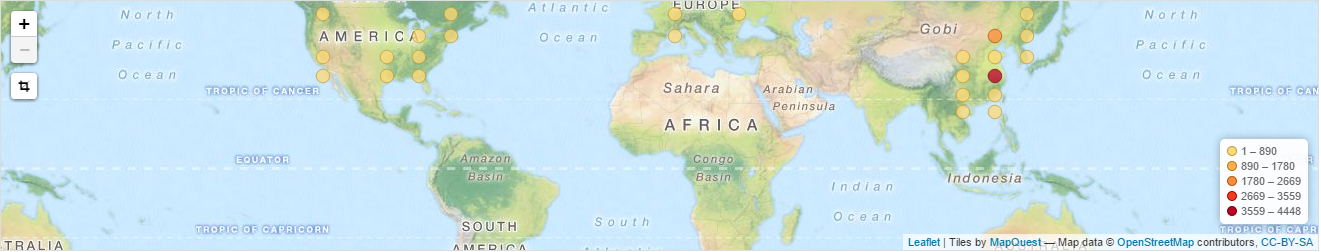
\includegraphics[width=0.9\linewidth]{images/map}
\end{figure*}


% TODO mention IPS data
\begin{figure*}[ht]
    \begin{subfigure}[ht]{0.5\linewidth}
        \caption{Infected IPs per ISP}
    \centering
    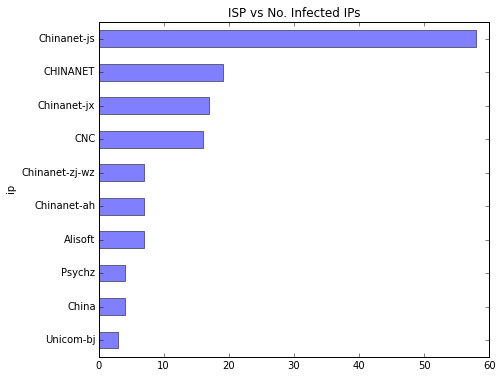
\includegraphics[width=\linewidth]{images/isp_no_ip}
    \end{subfigure}
\quad
    \begin{subfigure}[ht]{0.5\textwidth}
    \caption{BNI attempts per ISP}
    \centering
    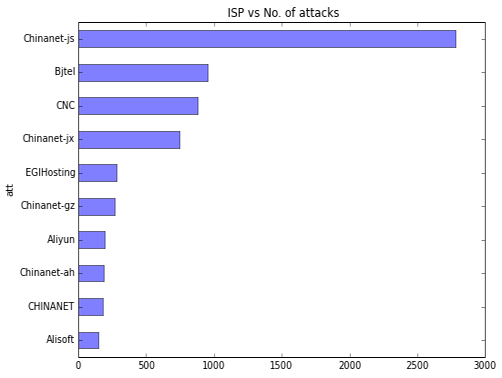
\includegraphics[width=\linewidth]{images/isp_no_att}
    \end{subfigure}

\end{figure*}
